%Modelowanie zjawisk elektromagnetycznych realizowane jest poprzez rozwiązywanie równań Maxwella dla oceny interakcji fal elektromagnetycznych z~obiektami fizycznymi i~otoczeniem. Wiele realnych problemów elektromagnetycznych nie jest rozwiązywalnych na drodze analitycznej, ze względu na nieregularności geometryczne spotykane w~strukturach czy trudne do analitycznego opisu właściwości elektromagnetyczne wykorzystywanych materiałów.

Poza zjawiskami kwantowymi i~nieliniowymi, zachowanie światła opisuje się przy użyciu liniowych równań Maxwella. Rozwiązywanie równań Maxwella jest w~ogólności niezmiernie złożone, a~jedynie dla bardzo prostych układów znane są ich rozwiązania analityczne. Z tego względu, tam gdzie jest to możliwe, równania Maxwella upraszcza się do skalarnego równania Helmholtza lub dalej do równania propagacji wiązki, albo do praw optyki geometrycznej. Odwołująca się do optyki geometrycznej metoda śledzenia promieni~(ang.~ray tracing) wykorzystana została w~tej pracy jedynie w~charakterze pomocniczym w~rozdziale 5, dotyczącym propagacji nadrozdzielczej w~ośrodku o~bardzo wysokiej efektywnej anizotropii. 

Ponadto wykorzystuje się uproszczenia wynikające z~symetrii układu oraz redukcji wymiarowości w~odpowiednio dobranym układzie współrzędnych. Częstym uproszczeniem jest zastąpienie bardziej złożonego układu prostszym, na przykład trójwymiarowego - dwuwymiarowym, lokalnie scharakteryzowanym efektywnym współczynnikiem załamania. Dodatkową korzyścią wynikającą ze sprowadzenia trójwymiarowego modelu układu do postaci planarnej jest możliwość użycia opisu skalarnego, wynikająca z~rozsprzęgnięcia równań Maxwella na polaryzacje TE~(ang.~transverse electric) i~TM~(ang.~transverse magnetic) zachodzące dla układów planarnych. W~dalszej części rozdziału, omówiony zostanie model ośrodka efektywnego dla struktur cienkowarstwowych.

\begin{figure}[tb]
	\centering
	\begin{subfigure}{0.45\textwidth}
		
\includegraphics[width=\textwidth]{images/wstep/fdtd.png}
		\caption{}
		\label{fig:wstep-fdtd-dic}
	\end{subfigure}
	\begin{subfigure}{0.45\textwidth}
		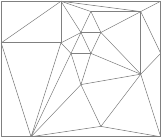
\includegraphics[width=\textwidth]{images/wstep/fem.png}
		\caption{}
		\label{fig:wstep-fem-dic}
		
	\end{subfigure}
	\caption{Porównanie siatek dyskretyzacji dla metody (a) różnic skończonych (ang. finite-difference) , (b) elementu skończonego (ang. finite-element, FEM)}
\end{figure}

Metody elektrodynamiki obliczeniowej~\cite{bondeson2005computational} odnoszące się do rozwiązywania równań Maxwella, tradycyjnie dzieli się na metody z~czasem i~metody sformułowane w dziedzinie częstości. Dla układów liniowych, w konsekwencji obowiązywania zasady superpozycji w~optyce, oba podejścia pozwalają uzyskać równoważne rozwiązanie problemu. Metody częstotliwościowe pozwalają na bezpośrednie wykorzystanie danych literaturowych opisujących dyspersję materiałową – zarówno w~odniesieniu do współczynnika załamania jak i~ekstynkcji. W~odniesieniu do pól monochromatycznych, w~oczywisty sposób są też znacznie szybsze od metod czasowych, co spowodowane jest brakiem konieczności uwzględnienia wymiaru czasowego w~symulacji. W~odróżnieniu od metod częstotliwościowych, metody czasowe np.~FDTD pozwalają jedynie na zastosowanie prostych modeli dyspersji np.~modelu Drudego i Lorenza dla dielektryków lub półprzewodników. Większość wyników opisanych w~tej pracy otrzymano w drodze bezpośredniego rozwiązania równań Maxwella omówionymi dalej metodami FDTD~(ang.~finite difference time domain method)~\cite{taflove1995computational} i~metodą macierzową TMM~(ang.~transfer matrix method). Pierwsza z~nich jest przykładem metody czasowej, druga zaś częstotliwościowej, o charakterze quasi-analitycznym. 

Poza podziałem na metody częstotliwościowe i czasowe oraz podziałem ze względu na użyte przybliżenia i~związany z~nimi wybór postaci równania i~warunków brzegowych, ważny podział odnosi się do sposobu dyskretyzacji pola i~regularności siatki obliczeniowej. W metodach modowych, pole aproksymuje się przez superpozycję rozwiązań. Jest tak na przykład w metodzie RCWA~(ang.~rigorous coupled wave analysis)~\cite{hench2008rcwa} stosowanej do opisu periodycznych siatek o złożonej budowie lub metodach macierzowych TMM/SMM~(ang.~transfer matrix method/scattering matrix method)~\cite{teich1991fundamentalsTMM,yeh2006} pozwalających na bardzo wydajne obliczenia współczynników transmisji i odbicia dla struktur warstwowych. W~metodach opartych na metodzie różnic skończonych~(np.~FDTD oraz niektórych sformłowaniach metody propagacji wiązki BPM) siatka dyskretyzacji ma zwykle postać regularną, najczęściej związaną z kartezjańskim lub walcowym układem współrzędnych. Inaczej jest natomiast dla metody elementu skończonego FEM (lub elementów skończonych, ang.~finite element method), w której funkcja falowa jest lokalnie interpolowana w zasadzie na dowolnej siatce, najczęściej wynikającej z odpowiedniej triangularyzacji układu. Nieregularność siatki powoduje, że metoda ta jest szczególnie użyteczna w odniesieniu do modelowania układów wymagających precyzyjnego oddania zjawisk zachodzących w różnych skalach, np. propagacji pola w przestrzeni swobodnej oraz wzbudzania powierzchniowych plazmonów polarytonów.

%Jednym ze sposobów na rozwiązywanie problemów elektromagnetycznych jest dyskretyzacja przestrzenna interesującego nas obszaru i~rozwiązanie równań Maxwella dla każdego punktu dyskretyzacji\footnote{Podejście to może wymagać znaczącej mocy obliczeniowej, oraz pamięci operacyjnej wykorzystywanych komputerów. Szczególnie w~symulacjach trójwymiarowych w~których dwukrotne zwiększenie rozdzielczości powoduje ośmiokrotny wzrost wymaganej pamięci RAM. }. Możemy wyróżnić dwa zasadnicze sposoby wprowadzenia siatki dyskretyzacji:
%\begin{itemize}
%\item Metodę różnic skończonych, w~której kolejne punkty obliczeniowe rozłożone są na ortogonalnej siatce równo oddalonych od siebie punktów. Ten sposób podziału obszaru obliczeniowego wiąże się z~trudnościami w~oddaniu nieprostokątnych kształtów geometrycznych, oraz niedokładnym odwzorowaniem obiektów, których rozmiary nie pasują do siatki dyskretyzacji. Tego typu siatkę przedstawia rysunek \ref{fig:wstep-fdtd-dic}.
%\item Metodę elementów skończonych. Przykładową siatkę dyskretyzacji przedstawia rysunek \ref{fig:wstep-fem-dic}. W przypadku metod  FEM~(ang. finite-element method) samo tworzenie odpowiedniej dyskretyzacji na podstawie definicji geometrii lub zdjęcia struktury może być zagadnieniem wymagającym obliczeniowo. Właściwy dobór siatki dyskretyzacji jest szczególnie ważny ze względu na większe (w porównaniu do siatki regularnej) możliwości występowania artefaktów numerycznych.  
%\item Metody w~których obliczenia nie są prowadzone na dyskretnej siatce. Jak omówiona w~rozdziale \ref{subart:tmm} metoda macierzy przejścia.
%\end{itemize}

Stosując metody obliczeniowe w dziedzinie czasu, wprost poszukujemy wartości składowych pól $E$ i~$H$ dla kolejnych chwil. Podstawową metodą obliczeniową wykorzystywaną w niniejszej pracy jest metoda różnic skończonych w~dziedzinie czasu opisana szeroko w~podrozdziałach \ref{subart:fdtd} - \ref{subart:borfdtd}. Największą zaletą takiego podejścia jest możliwość zadania dowolnych prądów $J(\vec{x},t)$, przez co sama symulacja staje się sensu stricte eksperymentem numerycznym. Metody tego typu są jednak bardzo wymagające obliczeniowo, w~szczególności dla symulacji trójwymiarowych dwukrotne zwiększenie gęstości siatki powoduje szesnastokrotne wydłużenie obliczeń. 

\subsection{Metoda propagacji wiązki} 

Metoda propagacji wiązki~(ang. beam propagation method - BPM)~\cite{scarmozzino2000numerical,van1981beam} jest przykładem metody w której rozwiązaniu numerycznemu poddawany jest problem wcześniej uproszczony na drodze analitycznej. W przypadku BPM, rozwiązaniu numerycznemu podlega równanie Helmholtza w~postaci:
\begin{equation}
 ( \nabla ^2 + k_0^2 n_^2) \Psi = 0,
\end{equation}
w którym $\Psi$ jest jedynie funkcją położenia powstałą w~wyniku założenia rozwiązań pola E-M w~postaci skalarnej $E(\vec{x},t)=\Psi(\vec{x})\cdot exp(-i\omega t)$. W dalszej części wyprowadzenia zakładamy, że pole można wyrazić przez iloczyn wyrażenia harmonicznego odpowiedzialnego za propagację w wyróżnionym kierunku $x_2$ i amplitudy pola $A(x1,x2)$:
\begin{equation}
\Psi(\vec{x})=A(x_1,x_2) exp\{ik_0\nu x_2\}, 
\end{equation}
gdzie gdzie $\nu$ jest parametrem dobranym w taki sposób, aby amplituda $A$ była słabo zmienna względem $x_2$. Podane założenie, o~wolnozmiennej obwiedni amplitudy, prowadzi do ostatecznego równania rozwiązywanego numerycznie w~metodzie BPM:
\begin{equation}
 \Big{  \frac{\partial^2 }{\partial x_1^2 } + (n^2 - \nu^2) \Big} A(\vec{x}) = \pm  2ik_0\nu \frac{\partial A (\vec{x})}{\partial x_1}.
\end{equation}

Metoda BPM polega na rozwiązaniu powyższego równania poprzez wyznaczenie rozkładu amplitudy A w kolejnych warstwach otrzymanych poprzez dyskretyzację w kierunku x2. Można to uzyskać stosując bezpośrednio metodę różnic skończonych i~schemat Crancka-Nicholsona, bądź poprzez przekształcenie powyższego równania przy użyciu dyskretnej transformaty Fouriera do reprezentacji widmowej we współrzędnej $x_1$. Wprowadzone przybliżenia, w~stosunku do bezpośredniego rozwiązywania równań Maxwella, zmniejszają złożoność obliczeniową metody BPM w~porównaniu z~bardziej rygorystycznymi algorytmami, prowadzą jednocześnie do ograniczeń takich jak brak możliwości symulacji struktur z~dużą zmiennością geometryczną w kierunku propagacji, konieczność iteracyjnej implementacji odbić, czy trudności z~symulacjami, w~których fala E-M propaguje się pod dużymi kątami względem osi układu optycznego.



 
